\documentclass[border=5pt]{standalone}
\usepackage{tikz}
\usetikzlibrary{calc}
\begin{document}
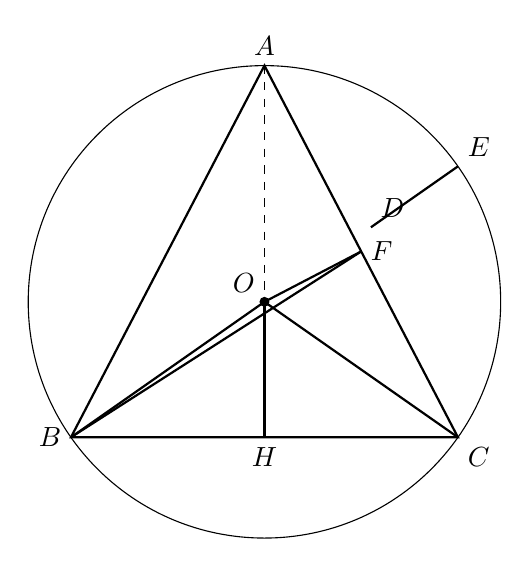
\begin{tikzpicture}[scale=1.5]
% Circle and center
\coordinate (O) at (0,0);
\draw (O) circle (2);
\fill (O) circle (1.2pt);

% Points on circle
\coordinate (A) at (90:2);
\coordinate (B) at (215:2);
\coordinate (C) at (325:2);
\coordinate (E) at (35:2);

% H midpoint of BC
\coordinate (H) at ($(B)!0.5!(C)$);

% D on segment EO
\coordinate (D) at ($(E)!0.45!(O)$);

% F foot of perpendicular from O to AC
\coordinate (F) at ($(A)!(O)!(C)$);

% Triangle ABC
\draw[thick] (A) -- (B) -- (C) -- cycle;

% AH dashed
\draw[dashed] (A) -- (H);

% O to H
\draw[thick] (O) -- (H);

% Line B-O kept, D-E kept (segment D-O removed)
\draw[thick] (B) -- (O);
\draw[thick] (D) -- (E);

% O to C
\draw[thick] (O) -- (C);

% O to F with right angle mark
\draw[thick] (O) -- (F);
\draw ($($(F)!6pt!(O)$)!6pt!90:($(F)!6pt!(C)$)$ ) ($($(F)!6pt!(O)$)!0!($(F)!6pt!(C)$)$);

% B to F
\draw[thick] (B) -- (F);

% Labels
\node[above] at (A) {$A$};
\node[left] at (B) {$B$};
\node[below right] at (C) {$C$};
\node[above right] at (E) {$E$};
\node[above right] at (D) {$D$};
\node[above left] at (O) {$O$};
\node[below] at (H) {$H$};
\node[right] at (F) {$F$};
\end{tikzpicture}
\end{document}
